% -*- coding: utf-8; -*-
% vim: set fileencoding=utf-8 :

% The paper on using Luau telemetry to measure the effectiveness of type error reporting.

\documentclass[english,submission,cleveref]{programming}
%% use 'submission' for initial submission, remove it for camera-ready (see 5.1)

%%\overfullrule=1mm

%% BEGIN tobias pape 2021-11-06
% Why do we need this? To have headings in the abstract.
\makeatletter
\newcommand*\abstractpart[1]{\unskip\par\noindent{\firamedium\color{P@GrayFG}{#1}}\enspace}
\makeatother
%% END

\usepackage{alltt}
% Not sure why <Programming> is recommending non-standard tools
% \usepackage[backend=biber]{biblatex}
\usepackage{amssymb}
\usepackage{calc}
\usepackage{colortbl}
\usepackage{listings}
\usepackage{mathpartir}
\usepackage{pifont}
% Errors with
% ! Undefined control sequence.
% <argument> \l__siunitx_number_implicit_plus_bool 
% l.61 \begin{document}
% using Mac TeXlive 20230313_2
% \usepackage{siunitx}
\usepackage{tikz}
\usepackage{subcaption}
\usepackage{wasysym}
\usepackage{xcolor}
\usetikzlibrary{shapes.geometric}

%%%%%%%%%%%%%%%%%%
\paperdetails{
  %% perspective options are: art, sciencetheoretical, scienceempirical, engineering.
  %% Choose exactly the one that best describes this work. (see 2.1)
  perspective=scienceempirical,
  %% State one or more areas, separated by a comma. (see 2.2)
  %% Please see list of areas in http://programming-journal.org/cfp/
  %% The list is open-ended, so use other areas if yours is/are not listed.
  area={Data mining for programming, Telemetry},
  %% You may choose the license for your paper (see 3.)
  %% License options include: cc-by (default), cc-by-nc
  % license=cc-by,
}
%%%%%%%%%%%%%%%%%%

%%%%%%%%%%%%%%%%%%
%% These data are provided by the editors. May be left out on submission.
%\paperdetails{
%  submitted=2023-1-31,
%  published=2016-10-11,
%  year=2016,
%  volume=1,
%  issue=1,
%  articlenumber=1,
%}
%%%%%%%%%%%%%%%%%%

\begin{document}

\title{Type Error Telemetry at Scale}
% lean, lite, modest, non-intrusive, private, ...
% {Millions of Type Errors} = 72M forced strict, 1/2M type error is disappointing!
%% \subtitle{Impersonal Telemetry to Measure User Experience}

% Alphabetical order for authors?

\author[a]{Ben Greenman}
\authorinfo{(\email{benjamin.l.greenman@gmail.com}) is a postdoc at Brown University. He will be joining the University of Utah in Fall~2023.}
\affiliation[a]{Brown University, Providence, RI, USA}
% \orcid{0000-0001-7078-9287}

\author[b]{Alan Jeffrey}
\authorinfo{(\email{ajeffrey@roblox.com}) is a Principal Software Engineer at Roblox.}
% \orcid{0000-0001-6342-0318}
\affiliation[b]{Roblox, San Mateo, CA, USA}

\author[a]{Shriram Krishnamurthi}
% \orcid{0000-0001-5184-1975}
\authorinfo{(\email{shriram@brown.edu}) is the Vice President of Programming Languages (no, not really) at Brown University.}

\author[b]{Mitesh Shah}
\authorinfo{(\email{mshah@roblox.com}) is Senior Engineering Director, Programmability, at Roblox.}

%\renewcommand{\shortauthors}{...}

\newcommand{\code}[1]{\texttt{#1}}
\newcommand{\FILL}{\textbf{FILL}}
\newcommand{\dotscale}[1]{\scalebox{0.72}{#1}}
\newcommand{\wideas}[2]{\makebox[\widthof{#2}][l]{#1}}
\newcommand{\twoline}[2]{\parbox[s]{1.4cm}{\flushleft#1\newline#2}}
\newcommand{\chkYes}{\dotscale{\CIRCLE}}
\newcommand{\chkMaybe}{\wideas{\dotscale{\Circle}}{\chkYes}}
\newcommand{\chkNo}{\wideas{}{\chkYes}}
\newcommand{\pct}[1]{\SI{#1}{\percent}}
\newcommand{\percentile}[1]{{#1}th~percentile}
\newcommand{\modefont}[1]{\texttt{#1}}
\newcommand{\mnocheck}{\modefont{nocheck}}
\newcommand{\mnonstrict}{\modefont{nonstrict}}
\newcommand{\mstrict}{\modefont{strict}}
\newcommand{\zerowidth}[1]{\makebox[0pt][l]{#1}}
\newcommand{\stddev}[1]{[#1\textsc{k}]}
\newcommand{\gcell}[1]{\cellcolor{green!20}#1}
\newcommand{\ycell}[1]{\cellcolor{yellow!18}#1}
\newcommand{\ocell}[1]{\cellcolor{orange!29}#1}
\newcommand{\rcell}[1]{\cellcolor{red!30}$\!\!$#1$\!\!$}
\newcommand{\gbox}[1]{\colorbox{green!20}{#1}}
\newcommand{\ybox}[1]{\colorbox{yellow!18}{#1\vphantom{Ap}}}
\newcommand{\obox}[1]{\colorbox{orange!29}{#1\vphantom{Ap}}}
\newcommand{\rbox}[1]{\colorbox{red!30}{#1\vphantom{Ap}}}
\newcommand{\tefsfont}[1]{\textsc{#1}}
\newcommand{\tekey}{\tefsfont{te}}
\newcommand{\fskey}{\tefsfont{fs}}
\newcommand{\QALAN}{\FILL{} Alan:}

%%
%% The code below is generated by the tool at http://dl.acm.org/ccs.cfm.
%% Please copy and paste the code instead of the example below.

\begin{CCSXML}
<ccs2012>
<concept>
<concept_id>10002944.10011123.10010916</concept_id>
<concept_desc>General and reference~Measurement</concept_desc>
<concept_significance>500</concept_significance>
</concept>
</ccs2012>
\end{CCSXML}

\ccsdesc[500]{General and reference~Measurement}

\keywords{types, gradual typing, telemetry, user study, large-scale study}

\maketitle

\begin{abstract}
  \let\paragraph\abstractpart

  \paragraph{Context}
  %% What is the broad context of the work? What is
  %% the importance of the general research area?
  {Roblox Studio} lets millions of creators
  build interactive experiences by programming in a variant
  of Lua called Luau.
  The creators form a broad group, ranging from novices writing
  their first script to professional developers, thus Luau
  must support a wide audience.
  As part of its efforts to support all kinds programmers, Luau includes an
  optional, gradual type system and goes to great lengths to minimize false
  positive errors.

  \paragraph{Inquiry}
  %% What problem or question does the paper
  %% address? How has this problem or question been
  %% addressed by others (if at all)?
  Since Luau is currently being used by many creators, we want to collect their feedback
  to improve the language and, in particular, the type system.
  The standard way to collect feedback at a large scale from creators working on
  realistic projects is to deploy client-side telemetry; however, we must do
  so in a way that respects creators' privacy.
  Whatever telemetry we use to study the Luau language cannot include
  personally-identifiable information.
  For example, we cannot monitor source code or error messages as they
  may contain personal data.
  Finding ways to harness telemetry in a private way is the central research challenge.
  %% TODO awkward

  \paragraph{Approach}
  %% What was done that unveiled new knowledge?
  We designed and implemented a pseudonymized telemetry system for Luau.
  Telemetry records include a timestamp, a session id, a reason for sending,
  and a numeric summary of the most recent type analysis.
  This information lets us follow type analysis over time within a codebase
  without revealing private information.
  Over four months in Spring 2023, we deployed the telemetry system and collected
  1.5 million telemetry records.

  \paragraph{Knowledge}
  %% What new facts were uncovered? If the
  %% research was not results oriented, what new
  %% capabilities are enabled by the work?
  We present several findings about Luau.
  Some confirm hypotheses by the Luau team while others are rather surprising,
  but all findings support our claim that pseudonymized telemetry is a
  useful way to collect feedback.
  One of the less-surprising findings is that types are unpopular:
  there is an 100x gap between the number of untyped Luau sessions and the number
  of typed ones.
  One surprise is that the strict mode for type analysis is very conservative
  about interactions with data assets.
  Instead of using the flexible dynamic type, it uses a top type and requires
  creators to down-cast assets.
  Lastly, a reassuring finding is that type analysis rarely hits its internal
  limits on problem size.

  \paragraph{Grounding}
  %% What argument, feasibility proof, artifacts,
  %% or results and evaluation support this work?
  Our findings are supported by a publicly-available dataset
  of over 1.5 million telemetry records
  and by free software for analyzing the data.

  \paragraph{Importance}
  %% Why does this work matter?
  Luau is the first large-scale combination of gradual types and semantic
  subtyping.
  Beyond the immediate benefits to Luau,
  our findings about types and type errors have implications
  for adoption and ergonomics in other gradual languages.
  %% mention Elixir, Verse?
  FILL specifics.
  Our telemetry design is of broad interest, as it gathers useful
  data without exposing personal information.

\end{abstract}

\section{Introduction}
\label{s:introduction}

{Roblox} is a platform for {shared virtual experiences}, with
65~million Daily Active Users, and 14~billion hours of engagement in
April--June 2023.
There are over 5~million experiences available on the platform thanks to a
worldwide community of 3~million creators~\cite{corp.roblox.com}.

Creators build experiences using the
{Luau} programming language~\cite{luau-lang.org},
an extension of {Lua~5.1~\cite{lua}}.
The main addition in Luau is a static type system, which infers
types for all Luau programs on the fly, as creators modify the code.
These types are used primarily in type-driven tooling such as autocomplete and
API documentation~\cite{luau-autocomplete}; the typical creator is unaware
that a type system powers these tools.
However, creators may write their own types, and they can opt in
to receiving ype error reports.

As discussed in~\cite{bfj-hatra-2021},
the goals of the {Luau} type system are rather different from
a traditional type system, which focuses on compilation and memory safety.
{Luau} has a diverse user community, ranging from
students in code camps to professional development studios. These
creators have quite different needs, with different emphases on
enabling rapid creation and ensuring software quality.
{Luau} therefore supports three typing modes for user code:
the hands-off default \mnocheck{},
a relaxed \mnonstrict{} mode,
and a rigorous \mstrict{} mode.
Creators can switch between modes
gradually~\cite{st-sfp-2006,tfffgksst-snapl-2017}, one module at a time.

In this paper, we investigate methods for measuring the effectiveness
of the {Luau} type system in the development of {Roblox} scripts.
We want to collect measurements at a large scale, with thousands
of participants, and we must do so in a way that protects creators' privacy.
In comparison to prior work~(\cref{s:related}), which
with few exceptions~\cite{zhlbr-cc-2020,zhlbr-oopsla-2020,hlzbr-ecoop-2021} is either small in scale
or collects personally identifiable information~(PII),
we performed a large-scale study using pseudonymized \emph{telemetry}.

{Roblox Studio} has a telemetry system, which is used to gauge
the effectiveness of creation features. This system randomly
determines which sessions should report telemetry, and for those
sessions, reports telemetry records back with a summary of the
session. In the case of this study, the telemetry includes data on the
number of errors at various levels of granularity: in the current edit
range, in the current file, and in every file which was type
checked.

The telemetry data we analyzed does not contain any PII.
It has no source code;
 no source locations;
no error messages (which may contain source code);
no error messages;
no record of the creator's identity, locale, or IP address;
and no information about what creation the data came from.
Telemetry records are correlated by session, using a pseudonymized
session identifier.

Most users of {Roblox Studio} do not opt in to type error
reporting (\pct{90},~\cref{s:data}), and so they do not see the ``squiggly underlining'' that
indicates a type error site. Nonetheless, the type inference system
still runs in the background (since it drives autocomplete and other
type-based tools), letting us see which type errors would have
been reported and whether users fix these errors over time.

With this telemetry data, we investigate research questions about
the adoption and benefits of type analysis:
\begin{description}
  \item[RQ1.]
    How many creators use type analysis?
    How often do projects contain modules with different
    analysis modes?
    How often do creators turn analysis off?
  \item[RQ2.]
    For modules that use type analysis:
    which errors arise,
    how do creators respond,
    and which errors tend to persist despite subsequent edits?
  \item[RQ3.]
    What impact does type analysis have on the number of background type
    errors?
    For example, do background errors pile up in unanalyzed projects?
\end{description}

Beyond their immediate applications to {Luau},
answers to these questions have implications for the design
of gradual types~\cite{st-sfp-2006}, success types~\cite{lindahl2006practical},
and semantic subtyping~\cite{CF05:GentleIntroduction,Jef22:SemanticSubtyping}.
Luau represents the first large-scale combination of these features,
and lessons from this experience can inform future applications.

At a higher level, this paper is the first to use telemetry 
to study a typechecker.
It thus represents a step toward data-driven language design,
informed by many users' actual practice.
Our data captures over 340,000 sessions
that occured between February and April 2023
and includes 72 million type analysis errors.
By contrast to typical qualitative methods such as surveys and interviews, it
is not restricted to users' \emph{perceptions} about their work and it is not
limited to a small number of users.

FILL can stats answer questions that point-by-point analysis cannot?

\paragraph{Contributions}
\begin{itemize}
  \item
    Design of a low-overhead, (black-box / PII-safe / impersonal)
    telemetry method, that other
    researchers can build on.

  \item
    Lessons from millions of type errors about
    the adoption of strict type analysis,
    the usefulness of type errors,
    and \FILL{}.
    These findings are especially important for the
    gradual typing, success typing, and semantic subtyping communities.

  \item
    \FILL{} any surprises when doing the analysis?
    Note, no ML for analysis, we do not have a corpus of text.

\end{itemize}

The data and the analysis pipeline are freely available.
\FILL{} link.


\section{{Roblox} Context}
% https://create.roblox.com/docs/scripting/luau

\begin{figure}[t]\centering
  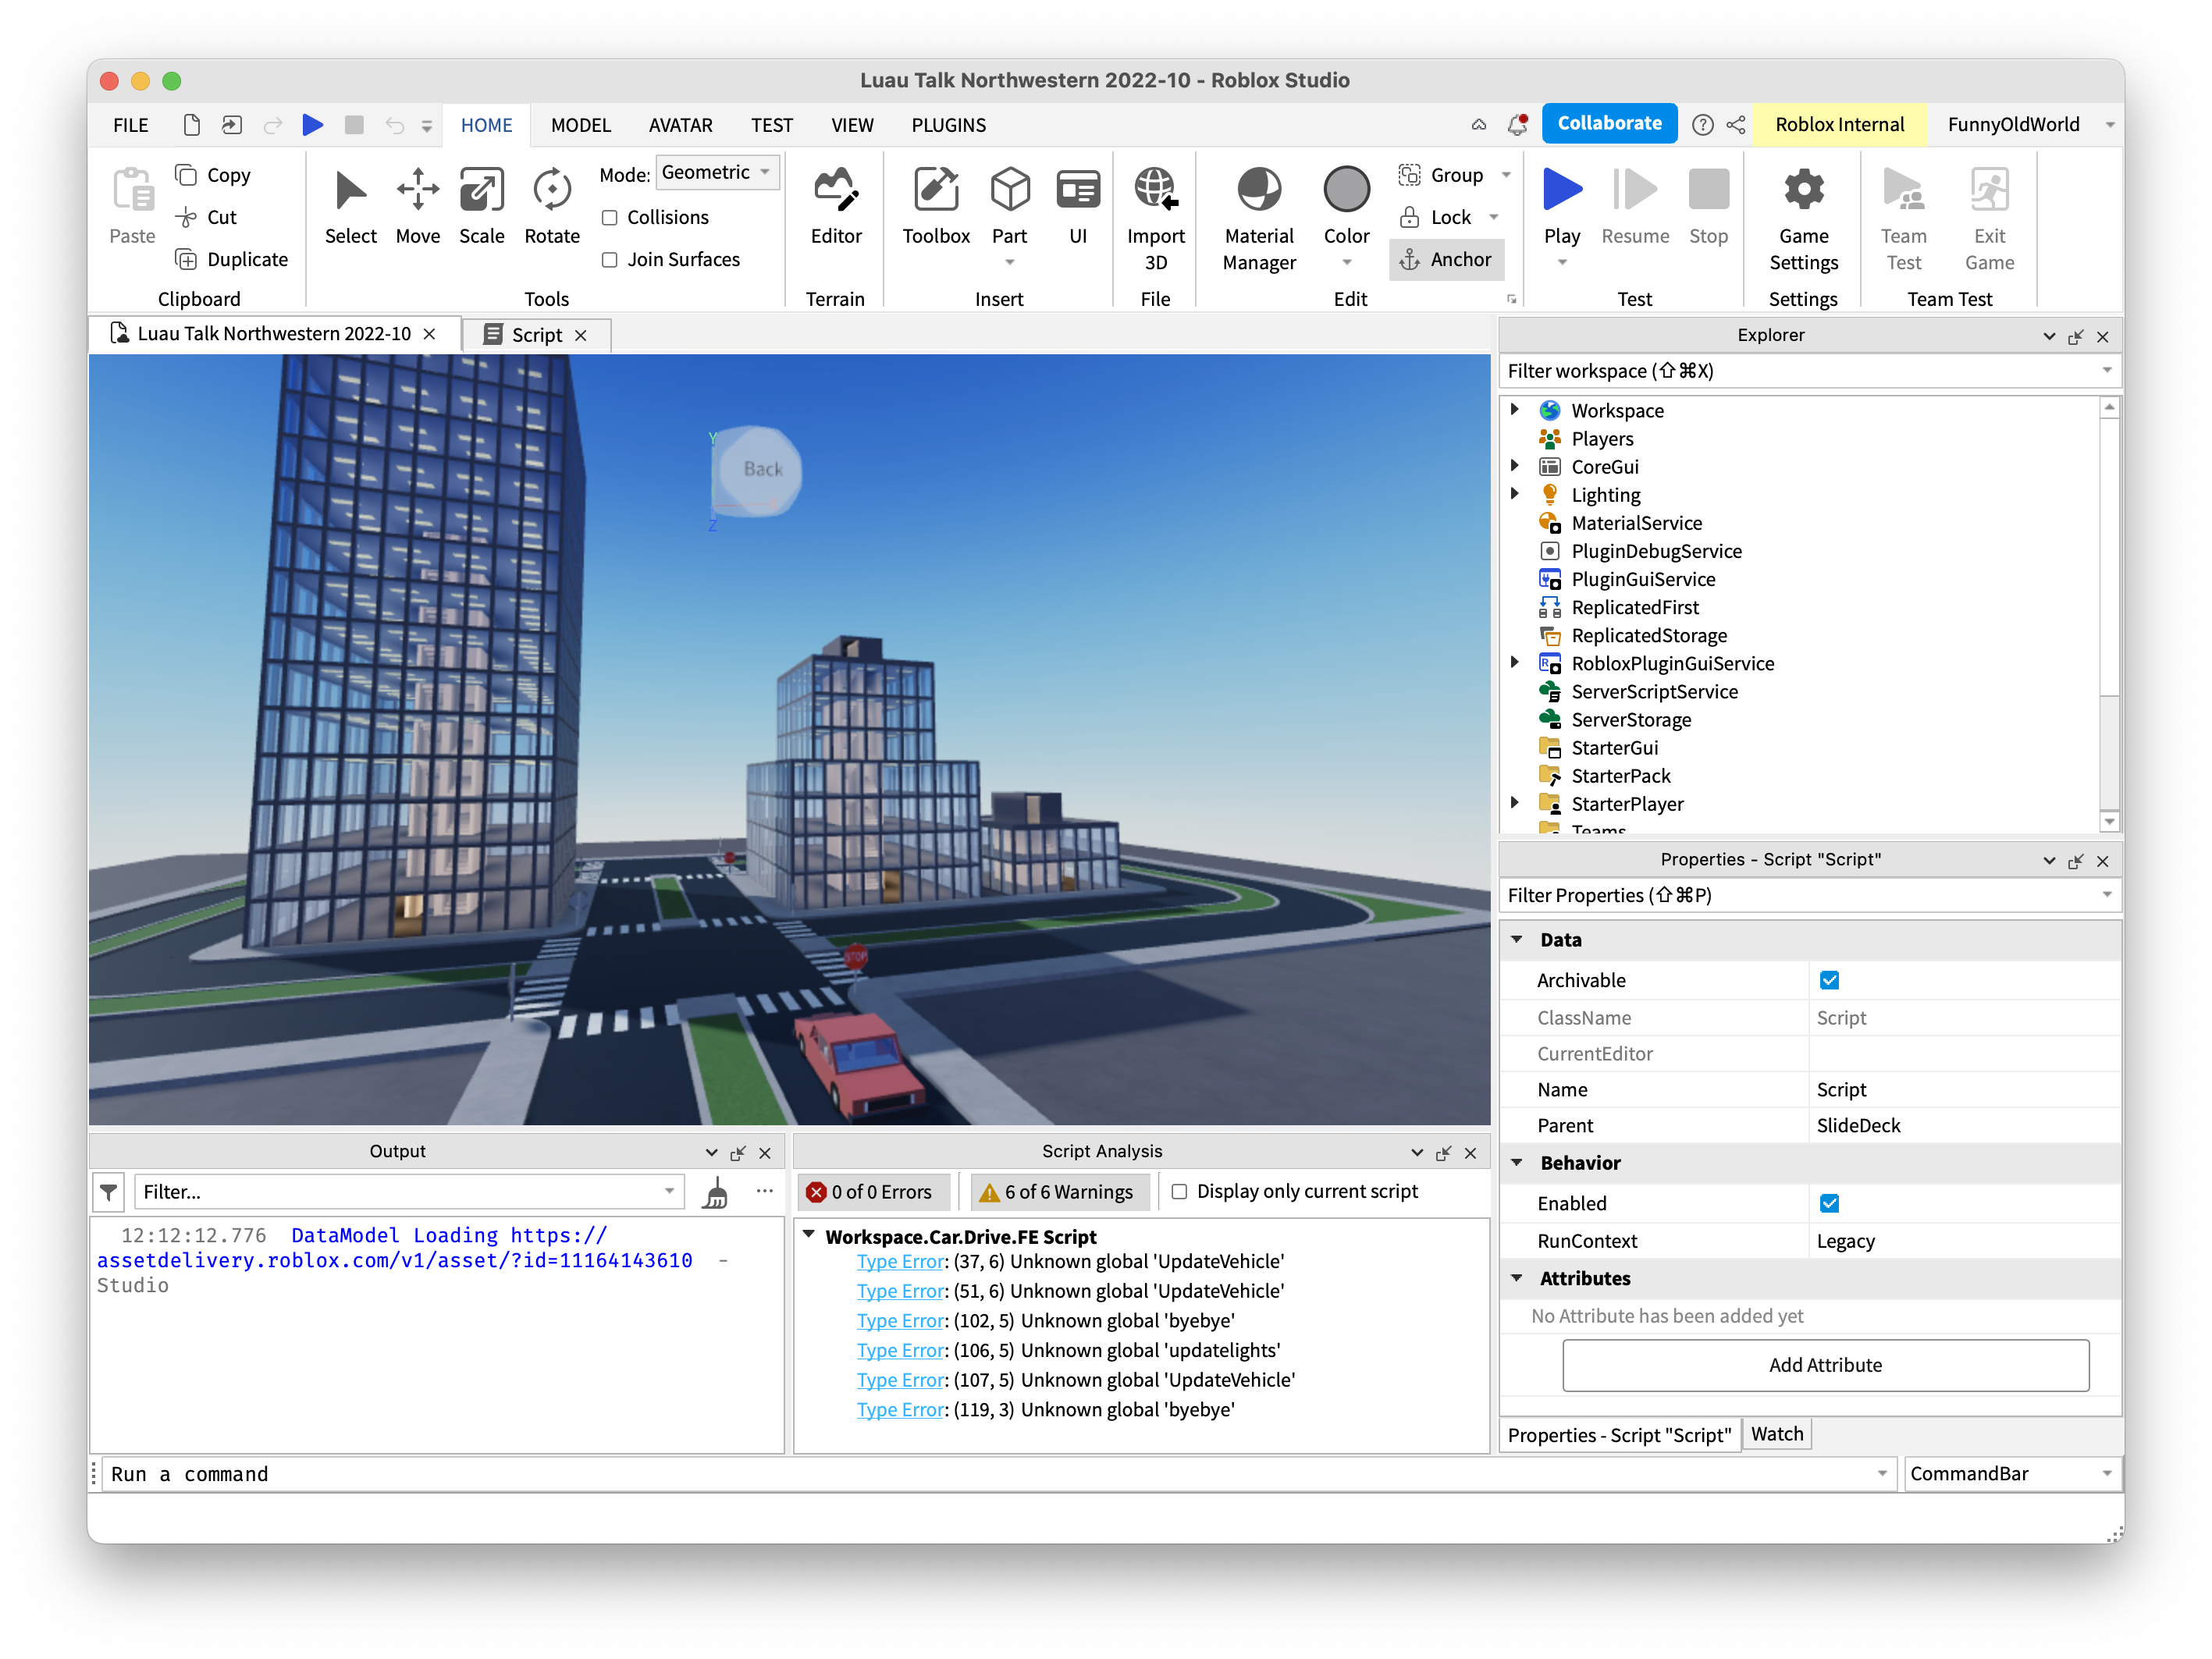
\includegraphics[width=.45\textwidth]{img/roblox-studio.png}
  \includegraphics[width=.45\textwidth]{img/roblox-studio-ide.png}

  \caption{{Roblox Studio 3D creation} tools (left) and IDE (right)}
  \label{fig:roblox-studio}
\end{figure}

%% \FILL{} explain the name "creators"?

{Roblox Studio} is a workbench that
combines {3D creation} tools and an Integrated
Developer Environment (IDE), as seen in \Cref{fig:roblox-studio}.
The IDE includes an optional ``Script Analysis'' widget, which
reports syntax errors, type errors, and problems identified by
lint tools. The script editor also (optionally) highlights
the location in code where reported errors occur.
To opt in to type error reporting, creators set a \emph{mode}
for each script, which is one of:
\begin{itemize}
  \item \mnocheck{}: only syntax errors are reported,
  \item \mnonstrict{}: all syntax errors, and a subset of ``high confidence'' type errors, are reported, or
  \item \mstrict{}: all syntax errors and type errors, are reported.
\end{itemize}
As an example of nonstrict mode, the following program only reports one error:
\begin{verbatim}
  --!nonstrict
  local x = { p = 5, q = nil }
  if condition then x.q = 7 end
  local y = x.p + x.q --> no type error
  local z = x.r       --> "Key 'r' not found in table 'x'"
\end{verbatim}
but in strict mode it reports two:
\begin{verbatim}
  --!strict
  local x = { p = 5, q = nil }
  if condition then x.q = 7 end
  local y = x.p + x.q --> "Type 'nil' could not be converted into 'number'"
  local z = x.r       --> "Key 'r' not found in table 'x'"
\end{verbatim}
In cases like this, where it is undecidable whether there will be a run-time error,
strict mode errs on the side of reporting an error, and nonstrict mode errs on
the side of suppressing the error.

Both modes report the \verb|Key 'r' not found in table 'x'| error --
misspellings of property names are common enough to report in both
strict and nonstrict mode. See~\cite{bfj-hatra-2021}
for a more detailed discussion of the rationale for strict and nonstrict mode.

Both modes are opt-in. The default for a new script is \mnocheck{} by
default, but creators can change this default to \mnonstrict{}.

Even in \mnocheck{} mode, {Roblox Studio} performs type inference, since
the results are needed by type-directed tooling such as autocomplete and
API documentation. This behind-the-scenes typechecking is always performed
in strict mode, since it is important that the inferred types be as precise
as possible. The type errors produced by this pass are always discarded,
so the verbosity of strict mode is not an issue.

Since this pass is always performed in strict mode, we refer to it as
\emph{forced strict} mode. Its main use is in autocomplete, so forced
strict mode is triggered on every keystroke

Scripts come in two favors: \emph{module scripts} and \emph{non-module
scripts}.  Module scripts provide reusable libraries, which may be
\emph{required} by other scripts. Since module scripts can require
other module script, modules form a graph (though it is
an error in strict mode if the graph is cyclic, and edges are removed to
make the graph acyclic).

When typechecking is performed for script analysis, any script that
has been modified is marked as dirty, then any script that is dirty,
or which transitively requires a dirty module, is typechecked. More
commonly, when typechecking is performed for autocomplete, only
the current script is typechecked, since it is the only dirty
script, and nothing it requires can transitively require it, since
the module graph is acyclic.

The state of the world in a {Roblox} experience is captured by
the \emph{data model}, which is a tree of \emph{instances}, such as
parts, models, meshes, effects, lighting, audio assets, and physics
constraints such as forces, springs and joints.
%% The data model can be seen in the Explorer view of~\Cref{fig:roblox-studio}.
%% ben: where is it? very hard to see
While an experience is under development, it is typical for the data
model to be edited (for example instances to be added, deleted, moved
or renamed). Since the initial shape of the data model tree is reflected in
the type system, it is possible for these edits to introduce type errors.

%% FILL table = object

\begin{table}
  \caption{Selected Error Labels}
  % https://github.com/Roblox/luau/blob/master/Analysis/include/Luau/Error.h
  %% from type analysis, but they're not all really type errors
  %% TODO review selection after analyzing the full data
  \label{t:type-error-labels}

  %% FILL examples for each error?
  \begin{tabular}{ll}
    Label & Interpretation \\\midrule
    \code{CodeTooComplex} & Type analysis failed, cannot understand the code\!\!\! \\
    %% \code{UnificationTooComplex} & Type analysis failed, unification solver hit a limit\!\!\! \\
    \code{SyntaxError} & Basic parse error, e.g., \code{for if end} \\

    \code{CountMismatch} & Arity mismatch for a function \\
    \code{IncorrectGenericParameterCount} & Arity mismatch for a generic type \\
    \code{UnknownProperty} & Referenced an invalid field or method  \\
    \code{OnlyTablesCanHaveMethods} & Tried to attach a method to a non-table \\
    \code{CannotCallNonFunction} & Called a value that is not a function \\
    \code{TypesAreUnrelated} & Failed to cast, unify, or check subtyping \\
    \code{TypeMismatch} & Generic label for other type errors \\
    \code{GenericError}
    & Generic label for other non-type errors, such as\\
    & \hbox{}~~looping over an unordered table
    %% attempting to extend a type that does not describe a class
    %% attempting to iterate over a table without a clear order


%    \code{ExtraInformation} & Follow-on error that provides additional information for an error at the same source location. \\
%    UnknownSymbol &  \\
%    NotATable &  \\
%    CannotExtendTable &  \\
%    DuplicateTypeDefinition &  \\
%    FunctionDoesNotTakeSelf &  \\
%    FunctionRequiresSelf &  \\
%    OccursCheckFailed &  \\
%    UnknownRequire &  \\
%    UnknownPropButFoundLikeProp &  \\
%    InternalError &  \\
%    DeprecatedApiUsed &  \\
%    ModuleHasCyclicDependency &  \\
%    IllegalRequire &  \\
%    FunctionExitsWithoutReturning &  \\
%    DuplicateGenericParameter &  \\
%    CannotInferBinaryOperation &  \\
%    MissingProperties &  \\
%    SwappedGenericTypeParameter &  \\
%    OptionalValueAccess &  \\
%    MissingUnionProperty &  \\
%    NormalizationTooComplex &  \\
%    TypePackMismatch &  \\
%    DynamicPropertyLookupOnClassesUnsafe &  \\)
  \end{tabular}
\end{table}

\section{Telemetry Design}

\subsection{Limits of telemetry}

Telemetry allows an application to ``phone home'' with data
summarizing usage patterns, such performance data, crash reporting,
and feature uptake. A typical usage is in deciding whether an API can
be deprecated: without telemetry it may be difficult to know how
popular a feature is with users, but with telemetry it is
straightforward.

IDEs use telemetry in a similar fashion to most user-facing
applications, for example VSCode~\cite{vsc-telemetry} and
IntelliJ~\cite{intellij-telemetry} report telemetry.
See~\cref{s:related} for futher comparisons among telemetry designs.

Telemetry for programming languages can be controversial, for example
the lively discussion around telemetry in the Go
toolchain~\cite{golang-telemetry}. 
The Luau open source toolchain does \emph{not} report telemetry,
as it is designed to be used in build environments such as Continuous Integration
servers, where hermetic deterministic builds are expected.

Much of the concern about telemetry is because of its potential impact on
privacy, by revealing Personally Identifiable Information (PII).
For this reason, it is important that any experiments using telemetry
not reveal PII:
no source code;
no source code locations;
no error messages (which may contain source code);
no record of the creator's identity, locale, or IP address;
and no information about what creation the data came from.
A good introduction to the privacy implications and tradeoffs
involved with telemetry is~\cite{transparent-telemetry}.

For performance reasons, there are limits to telemetry data:
telemetry records have size limits, and the performance impact of
recording telemetry should be minimal.

In summary, the limitations of telemetry are:
\begin{itemize}
  \item Data which reveals no PII.
  \item Fixed-size telemetry records.
  \item Minimal overhead to record telemtry.
\end{itemize}
In addition, due to the architecture of Roblox Studio
there is some information that is not available to the
typechecker:
\begin{itemize}
  \item The typechecker does not have access to some lifecycle events,
    such as save, quit and publish.
  \item The typechecker does not have access to GUI state, for example
    whether the Script Analysis widget is visible.
\end{itemize}

\subsection{Telemetry records}
\label{s:telemetry-records}

The telemetry for a Roblox Studio session is gathered as a series of
telemtry records, all with the same psedonynimized session
identifier. This allows us to correlate telemetry across a single
session, but not between sessions.

In order to avoid swamping our telemetry servers, we randomly throttle
the generation of telemetry records:
\begin{itemize}
  \item
    1\% of Roblox Studio sessions were enrolled in generating telemetry, and
  \item
    0.5\% of runs of the typechecker (approximately 1 in 200 keystrokes)
      in an enrolled session generated a telemetry record.
\end{itemize}
In order to find how file-switching correlated with type errors, we additionally have:
\begin{itemize}
  \item
    every run of the typechecker in an enrolled session which switched file generated a telemetry record.
\end{itemize}
Each telemetry record contains nine kinds of data:
\begin{enumerate}
  \item metadata: a psedonymized session identifier, timestamp and session duration,
  \item mode of the current file: (\mnocheck{}, \mnonstrict{}, or \mstrict{}),
  \item reason for sending: (random selection, or file switch),
  \item size of codebase: number of files, and number of lines of code type checked,
  \item size of edit range
  \item overall type errors: for previous and current states, we have the total number, the nunber in the current file, and number in the edit range,
  \item specific errors in the edit range: for the previous and current states, for each type error code, the number type errors in the edit range,
    \FILL{} explain previous/current in detail, explain that this data takes up most of the telemetry record
  \item forced strict errors: specific errors for the
    edit range computed as if the user had strict mode enabled.
  \item TooComplexErrors: project-wide count for this one specific error type
\end{enumerate}
To track the edit range, we record a start and end position, which we
update appropriately on every edit. This can result in very large edit
ranges, for example, if the user edits at the beginning and end of the
file.
The main benefit of this strategy is that it ensures constant-size telemetry records.


\section{The Data}
\label{s:data}

Roblox Studio collected type error telemetry in Spring 2023,
between February and April.
Every Studio session had a small random chance of generating
telemetry~(\cref{s:telemetry-records}).
The chosen sessions generated a record whenever the user switched modules and
randomly on each keystroke.
In total, we collected 1.5 million telemetry records.
Roughly two-thirds of records are due to keystrokes.

\Cref{f:records-per-hour} provides a time-ordered distribution of the data.
Each vertical bar counts the number of records generated per hour according to
a client-side timestamp.
The bars are labeled with a California time zone because that is the locale of
the Roblox servers, which parsed the timestamps.
Most buckets contain roughly one thousand records, but some have very few
and a handful of others exceed three thousand.
%% \FILL{} investigate one tower, what's happening?? all one session?
There is a sharp drop in early April when the experiment was finished
and the telemetry probe was removed (though there is a long tail as
developers uopdated Roblox Studio).
We do not know which timezone the records originated in, but since the counts
tend to peak midday California time it seems that the majority
of Roblox developers are following a Western Hemisphere schedule.
The counts for weekends (shaded regions) are often the tallest,
as Roblox has a significant school-aged creator community.

\begin{figure}[t]\centering
  %% TODO bigger text
  %% TODO weird artifact (|) in x-min label
  %% code/row-distribution.rkt
  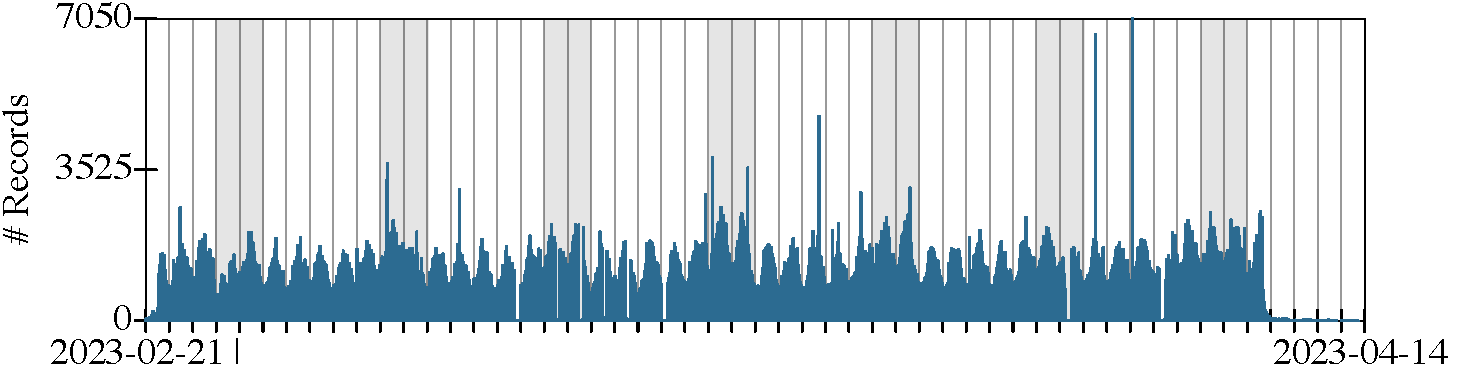
\includegraphics[width=\columnwidth]{img/row-distribution.pdf}
  \begin{tabular}{ll}
    Reason for sending:
    &
    \begin{tabular}[t]{r@{~~}l@{~~}r}
      996,164 & due to keystrokes  & [\pct{66.20}] \\
      508,572 & due to module switch & [\pct{33.80}]
    \end{tabular}
  \end{tabular}
  \caption{Telemetry records per hour. Each tick on the $x$-axis marks the start of a new day in California. Shaded ranges correspond to weekends.}
  \label{f:records-per-hour}
\end{figure}


\subsection{Data Cleaning}
\label{s:data-cleaning}

A close inspection of the data revealed a few anomalies.
For the most part, we omit the strange data from futher analysis.

First, some records have odd timestamps according to the server's records.
Every telemetry record comes with two timestamps: a client-side timestamp
from when Roblox Studio created it and a server-side timestamp from when
the server posted it to its database.
The server timestamps are little use for our analysis because they bunch
together; it is common for several records to have identical server
timestamps.
However, server timestamps are useful for auditing because they should
be relatively close in value to the client timestamps.
For a small number of records (<100? \FILL{}), though, the client is off by a large
margin: up to one week behind and up to one day ahead of the server.
We attribute the large delays to issues when sending telemetry (lost internet
connection, etc.) and smaller offsets to incorrect time settings on the client
machine.
In any event, we do not filter these records from further analysis.

Second, some records have identical (client) timestamps.
This can happen legitimately if type analysis runs several times
in the same millisecond, but it is unlikely that a human would
enter keystrokes or switch modules quickly enough.
We keep the first record with a distinct timestamp and discard the others.
%% TODO wait, better deduplicate by session and not globally!!!

%% out/negative-edit-range.txt
%% actual value is NOT negative, but large positive over 4 billion
%% example: 4294967293
Third, the edit ranges are negative in a few hundred records~(1,533).
This is likely due to the user deleting a large block of code.
Since the issue affects so few records, we omit the negative ranges
from analysis (but, we do use other parts of the records; for example
the timestamps influence~\cref{f:records-per-hour}).

\subsection{Overall Size and Shape}

The first step toward understanding the data is to have a sense of what
is in it.
Three important characteristics are the size of the codebases in the data,
the length of the sessions we captured, and the number of type analysis
errors.
We discuss these in turn.
Codebase size and session length follow power-law distributions, with
many small items and a few very large items.
The number of type analysis errors is somewhat low~(explained in the next
section), but sufficient to proceed with futher analysis.


\paragraph{Codebase Size}
%\label{s:codebase-size}

\begin{figure}[t]
  % ;; (list* (max* vv) (median < vv) mm (stddev/mean mm vv) (percentile* vv)))
  % ;; percentile* = 0.95 -- 0.99
  % #hash((editrange . (1156036 926 3007043/817 30975.40553032358 (0.95 8220) (0.96 9858) (0.97 13656) (0.98 18956) (0.99 34725)))
  %       (event-count . (6079 138 38689/135 582.5752201972966 (0.95 960) (0.96 1174) (0.97 1304) (0.98 1836) (0.99 3302)))
  %       (files . (54884 7678 55257996/4639 11853.650098459446 (0.95 40029) (0.96 42771) (0.97 45417) (0.98 48688) (0.99 51761)))
  %       (lines . (1089963 3115 38928947/5992 22364.75846303099 (0.95 18561) (0.96 25892) (0.97 27014) (0.98 29725) (0.99 50547)))
  %       (timespan . (1387897376 845648 591343604248/185705 15724745.722577972 (0.95 10696064) (0.96 12715468) (0.97 15596940) (0.98 21153924) (0.99 35450460))))
  %% NOTE: 3 records have +1M lines, all from one nocheck session, all with 3 files
  %% - session "30,762,216,447,324"
  %% NOTE: 133 records have +52K files, all from one nocheck session
  %% - session "330,172,870,224,081" 
  %% (2nd biggest has 41K files "31,650,473,913,529")

  \begin{tabular}{l@{}r@{~}l@{}r@{~}l@{}r@{~}l}
                 & Files  &              &     Lines &             &    Edit Range & \\
    Mean [std]   & 11,911 & \stddev{12}  &     6,497 & \stddev{22} &         3,680 & \stddev{31} \\
    Median       &  7,678 &              &     3,115 &             &           926 & \\
    \pct{99}     & 51,761 &              &    50,547 &             &        34,725 & \\
    %% TODO x-axis starts at 1, not zero ... there are no zeros right??!
    & 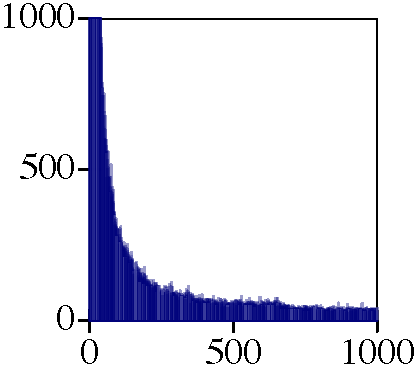
\includegraphics[width=0.2\columnwidth]{img/files-distribution.pdf}
    & & 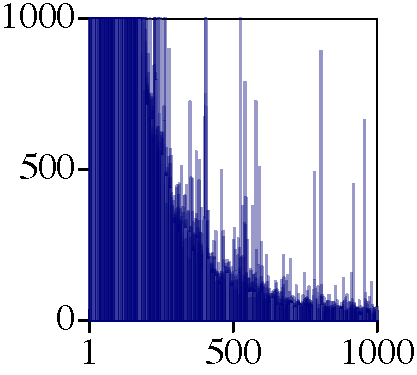
\includegraphics[width=0.2\columnwidth]{img/lines-distribution.pdf}
    & & 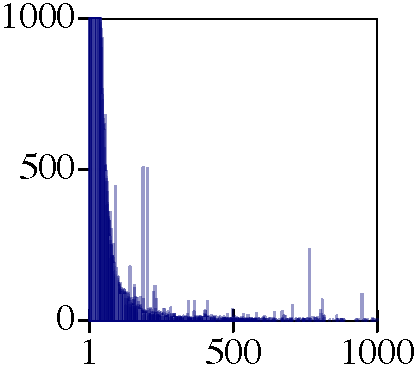
\includegraphics[width=0.2\columnwidth]{img/editrange-distribution.pdf}

  \end{tabular}

  \caption{Size of analyzed code: number of files, number of lines , and lines in edit range}
  \label{f:codebase-size}
\end{figure}

\Cref{f:codebase-size} summarizes the size of projects in the dataset.
The top half of the figure reports the mean, standard deviation, median,
and \percentile{99} for the number of files, lines, and lines in edit range.
The bottom half shows zoomed-in distributions of the file, line, and edit range
numbers.
For example, the x-axis of the first plot ranges from 0 to 1,000 files and
the y-axis counts up to 1,000 telemetry records.

There is a huge amount of variation across projects.
The largest ones have over 50,000 files, and
there are many small ones with 1 file and/or 1 line of code.
Unsurprisingly, the numbers come with large standard deviations.
The median values are more reasonable, with roughly 3,000 lines of code
and 1,000 lines in edit ranges, but still have a large number of files: over 7,000.
One source of variation is that some developers use Luau scripts as a way
to store data, writing a module that exports one huge array, typically
defined on a single line. Such data storage scripts provide a challenge for
script tooling.

%% The high number of files may be because creators define many components to
%% build a Roblox experience and put these components in separate files.
%% (\FILL{} still that's a lot of components ... any better guesses?)

%% (\FILL{} doublecheck file sizes)
% That seems way off, not sure we're seeing so many files :/

\paragraph{Session Size}
%\label{s:session-size}

\begin{figure}[t]\centering
  %% NOTE max time = 1 million seconds = 15 days ...  +100 are over 2 days

  \begin{tabular}{l@{}r@{~}l@{}r@{~}l} \\
                 & Time Span (sec)  &       & Record Count  \\
    Mean [std]   &     3,184 & \stddev{16}  &     286 & [583] \\
    Median       &       845 &              &     138        \\
    \pct{99}     &    35,450 &              &   3,302        \\
    %% TODO x-axis starts at 1, not zero ... there are no zeros right??!
    & 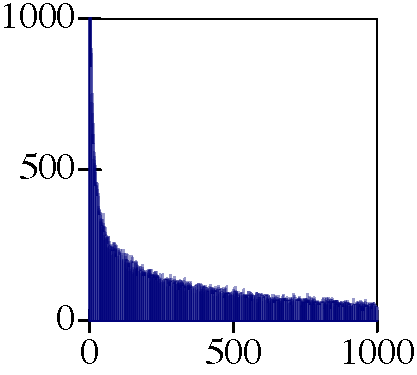
\includegraphics[width=0.2\columnwidth]{img/timespan-distribution.pdf}
    & & 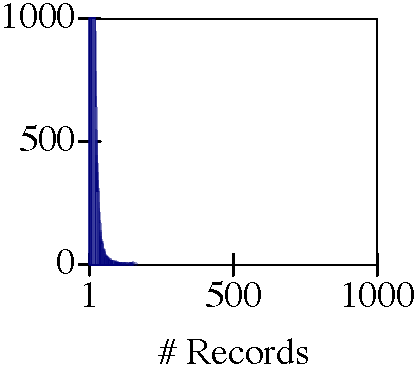
\includegraphics[width=0.2\columnwidth]{img/event-count-distribution.pdf}

  \end{tabular}

  \caption{Session size in seconds and in number of records}
  \label{f:session-size}
\end{figure}

\Cref{f:session-size} outlines the size of the Roblox Studio sessions in the
data.
There are two useful notions of size: real time in seconds (between the first
and last record) and the total number of records.
The top of~\cref{f:session-size} reports the mean, standard deviation,
median, and \percentile{99}; the bottom shows size distributions, zoomed in
to focus on at most 1,000 units (x-axis) and 1,000 sessions (y-axis).

Similar to the data on project size, there is huge variation in session
length.
The longest sessions last several days and/or contain thousands of records,
while the shortest last a few milliseconds or include just one record.
Likewise, both plots in the figure follow a power-law distribution
(especially for record count).
A typical session runs on the order of minutes and consists of a few dozen events.
The median session time is approximately 14 minutes.
The median number of
records is 138.
% These numbers are reasonable.


\paragraph{Number of Type Analysis Errors}
%\label{s:count-analysis-errors}

\begin{figure}[t]
  \begin{tabular}[t]{ll} \\
    \begin{tabular}[t]{l@{~~}r@{~}l}
      595,137 & type errors \\
      289,698 & in current module & [\pct{48.68}] \\
       30,924 & in edit range & [\pct{5.20}]
    \end{tabular}
    \begin{tabular}[t]{l@{~~}r@{~}l}
      72,235,735 & {forced strict errors} \\
      37,027,281 & in current module & [\pct{51.26}] \\
       1,111,178 & in edit range & [\pct{1.54}]
    \end{tabular}
  \end{tabular}
  \caption{Type errors and forced strict errors across all telemetry records}
  \label{f:count-analysis-errors}
\end{figure}

\FILL{} need old and current in edit range

\Cref{f:count-analysis-errors} lists the number of type analysis errors
and breaks them down by location in the codebase.
In total, there are nearly 600K type errors.
These appeared in modules that opted in to typechecking with either the
\mnonstrict{} or \mstrict{} mode.
The number of forced strict errors is much larger, 72M, because this analysis
ran on every module using strict type.
(Furthermore, forced strict runs silently, so creators have no incentive to
fix these errors.)
Approximately half the analysis errors occurred in the current module,
and a small fraction overlapped with the current edit range~(\pct{5} for
type errors, \pct{1} for forced strict).

The large fraction of errors in the current module is encouraging.
It suggests that errors appear locally, as the result of edits to nearby
code (as opposed to edits in one module raising errors in another), and
that creators fix the errors before switching focus to another
module.
The low fraction of errors in the edit range suggests that errors rarely
persist through nearby edits.


\subsection{Type Analysis Modes}
\label{s:type-analysis-modes}

\begin{figure}[t]\centering
  \begin{subfigure}[t]{\columnwidth}
    \begin{tabular}[t]{ll}
      %% FILL bar chart? rectangle?
      \begin{tabular}[t]{r@{~~}l@{~}r}
         1,341,348 & \mnocheck{}          & [\pct{89.14}] \\
           156,883 & \mnonstrict{}        & [\pct{10.43}] \\
             6,505 & \mstrict{}           & [\pct{ 0.43}]
      \end{tabular}
      \begin{tabular}[t]{r@{~~}l@{~~}r}
      \end{tabular}
    \end{tabular}
    \caption{Analysis modes across the 1,504,736 records}
    \label{f:total-records}
  \end{subfigure}

  \begin{subfigure}[t]{\columnwidth}
    \begin{tabular}[t]{ll} \\
      \begin{tabular}[t]{l@{~~}r@{~}l}
        313,509 & \mnocheck{}   & [\pct{90.19}] \\
         32,902 & \mnonstrict{} & [\pct{ 9.47}] \\
            545 & \mstrict{}    & [\pct{ 0.16}] \\
            642 & mixed-mode    & [\pct{ 0.18}]
      \end{tabular}
      \begin{tabular}[t]{l@{~~}ll}
        \zerowidth{Among the mixed-mode sessions:} \\
        & 341 & contain a mode upgrade \\
        & 320 & contain a mode downgrade \\
        & 512 & contain modules with different modes
      \end{tabular}
    \end{tabular}
    \caption{Analysis mode(s) for the 347,598 sessions}
    \label{f:total-sessions}
  \end{subfigure}

  \caption{Overview of type analysis modes}
  \label{f:dataset-overview}
\end{figure}

Creators have three analysis modes to choose from.
Furthermore, they can switch between modes at any time.
According to~\cref{s:type-analysis-modes}, however, usage is
extremely skewed toward the type-free \mnocheck{} mode.
Nearly \pct{90} of all records use the \mnocheck{} mode
and \pct{90} of all sessions use \mnocheck{} exclusively.
Among the rest, roughly \pct{10} of all records use \mnonstrict{} and only a
tiny fraction (\pct{0.4}) use \mstrict{}.
The per-session data is similar: \pct{9} use \mnonstrict{} exclusively
and \pct{0.2} use \mstrict{}.

These adoption numbers indicate that there is a communication gap;
as long as type checking is opt-in, most developers stay opted out.
Once Luau type checking is opt-out rather than opt-in, it will be interesting
to revisit these numbers.

%% mostly pure, rare mixes
Most sessions (\pct{99.82}) stick to a single analysis mode.
These sessions never change the mode in the current module and never switch
focus to a module with a different analysis mode.
Among the mixed-mode sessions, most (\pct{80}) switch to modules with
a different mode, about half contain at least one edit that upgrades the
current mode, and about half contain a downgrade.
There are 619 upgrades in total and 583 downgrades.
\FILL{} Ben check how often the downgrades follow the upgrades.


\paragraph{Are Upgrades Discouraging?}

%% 619 up-pairs, 583 down-pairs
%% === UP
%% min -3 max 57 median 0 mean 2.62 stddev 6.8390518952707335
%% === DOWN
%% min -48 max 30 median 0 mean -0.31 stddev 4.498748355271854

A possible explanation for the low adoption of \mnonstrict{} and
\mstrict{} mode is that upgrading to these modes leads to a large
number of type errors.
Creators might get discouraged by a high error count and revert to
\mnocheck{} mode.

The data does not support this explanation.
On average, the mode-upgrades in the data resulted in 3 additional
type errors (stddev 7, median 0).
The worst-case increase was 57 type errors, which is very high
but exceptional.
In another exception, upgrading modes removed three type errors
(possibly due to other edits being rolled in with the
mode change).

Similarly, mode downgrades have only a small negative effect on the
number of errors (mean -0.3, stddev 4, median 0, max -48).
%% curious outlier: downgrade added 30 errors!
Creators apparently tend switch modes only when the code is already
well typed, or close to it.


%% \paragraph{Module Switches vs Errors}
%% FILL need \%s out of all module switches.
%% How many module switches exit a module with errors?
%% > OLD DATA
%% > \mnocheck{} 24, \mnonstrict{} 9, \mstrict{} 3.
%% > Rare?
%% > More common for forcedstrict:
%% >  \mnocheck{} 190, \mnonstrict{} 16, \mstrict{} 2.
%% >
%% > How many module switches go to a module with errors?
%% > \mnocheck{} 70, nonstrict 9, strict 4
%% > For FS: \mnocheck{} 400, \mnonstrict{} 39, \mstrict{} 6.


\subsection{Type Errors vs. Program Edits}
\label{s:type-error-survival}

\begin{table}[t]
  \caption{Number of records that add, keep, or drop (remove) specific type errors from their edit range.}
  \label{t:type-error-survival}
  \begin{tabular}{lr@{}r@{}rr@{}r@{}rr@{}r@{}r}
    & \zerowidth{\mnocheck{}} & & & \zerowidth{\mnonstrict{}} & & & \zerowidth{\mstrict{}} & & \\
    & \rbox{Add} & \ybox{Keep} & \gbox{Drop} & \rbox{Add} & \ybox{Keep} & \gbox{Drop} & \rbox{Add} & \ybox{Keep} & \gbox{Drop} \\\midrule
    \code{CannotCallNonFunction} & {0} & {0} & {0} & {17} & {4} & {20} & {1} & {0} & {1} \\
    \code{CannotExtendTable} & {0} & {0} & {0} & {7} & {9} & {10} & {0} & {0} & {1} \\
    \code{CannotInferBinaryOperation} & {0} & {0} & {0} & {1} & {2} & {1} & {7} & {6} & {9} \\
    \code{CountMismatch} & {0} & {0} & {0} & {223} & {48} & {269} & {12} & {2} & {17} \\
    \code{DuplicateTypeDefinition} & {0} & {0} & {0} & {1} & {0} & {0} & {0} & {0} & {0} \\
    \code{ExtraInformation} & {0} & {0} & {0} & {48} & {7} & {39} & {2} & {0} & {1} \\
    \code{FunctionDoesNotTakeSelf} & {0} & {0} & {0} & {4} & {6} & {5} & {0} & {0} & {0} \\
    \code{FunctionExitsWithoutReturning} & {0} & {0} & {0} & {9} & {3} & {6} & {11} & {5} & {8} \\
    \code{GenericError} & {0} & {0} & {0} & {206} & {52} & {203} & {8} & {1} & {9} \\
    \code{IllegalRequire} & {0} & {0} & {0} & {16} & {3} & {33} & {0} & {0} & {2} \\
    \code{IncorrectGenericParameterCount} & {0} & {0} & {0} & {0} & {0} & {0} & {1} & {0} & {1} \\
    \code{MissingProperties} & {0} & {0} & {0} & {11} & {3} & {11} & {6} & {4} & {6} \\
    \code{MissingUnionProperty} & {0} & {0} & {0} & {1} & {0} & {2} & {0} & {0} & {0} \\
    \code{ModuleHasCyclicDependency} & {0} & {0} & {0} & {20} & {9} & {15} & {0} & {0} & {1} \\
    \code{NotATable} & {0} & {0} & {0} & {7} & {2} & {8} & {2} & {0} & {1} \\
    \code{OccursCheckFailed} & {0} & {0} & {0} & {0} & {0} & {0} & {0} & {0} & {1} \\
    \code{OnlyTablesCanHaveMethods} & {0} & {0} & {0} & {1} & {0} & {2} & {0} & {0} & {0} \\
    \code{OptionalValueAccess} & {0} & {0} & {0} & {40} & {52} & {27} & {6} & {2} & {7} \\
    \code{SyntaxError} & {8349} & {314} & {19220} & {983} & {46} & {2658} & {16} & {0} & {71} \\
    \code{TypeMismatch} & {0} & {0} & {0} & {159} & {62} & {129} & {21} & {10} & {28} \\
    \code{TypesAreUnrelated} & {0} & {0} & {0} & {1} & {0} & {0} & {0} & {0} & {1} \\
    \code{UnknownPropButFoundLikeProp} & {0} & {0} & {0} & {26} & {18} & {21} & {1} & {0} & {1} \\
    \code{UnknownProperty} & {0} & {0} & {0} & {347} & {180} & {385} & {19} & {19} & {35} \\
    \code{UnknownRequire} & {0} & {0} & {0} & {91} & {39} & {85} & {12} & {3} & {4} \\
    \code{UnknownSymbol} & {0} & {0} & {0} & {2348} & {496} & {2973} & {49} & {19} & {55}
  \end{tabular}

\end{table}

Equipped with an overall picture of the dataset and the skewed usage
of \mnocheck{}, \mnonstrict{}, and \mstrict{} modes, we are ready to explore
the type error data.
Our main focus is on the intersection between type errors
and edits to the programs.
When a type error highlights part of the code and the next edit range includes
that code, we want to know whether the error survives the edit.
Similarly, we want to know when an edit introduces a type error.

\Cref{t:type-error-survival} counts the number of times that types
errors overlap with the current edit range.
There are three sets of columns, corresponding to the \mnocheck{},
\mnonstrict{}, and \mstrict{} type analysis modes.
Within each set, the Add columns counts the number of telemetry records
that introduce a certain type error.
For example, seventeen of the \mnonstrict{} records add
at least one \code{CannotCallNonFunction} error to the current edit range.
The Keep columns counts records that have the same, non-zero number of type errors
before and after.
Lastly, the Remove columns count records that decrease the number of type errors.

All three counts are imprecise because our telemetry does not track the exact
identity of a type error.
Suppose a creator removes one \code{CannotCallNonFunction} error but then
immediately introduces another on a different line.
\Cref{t:type-error-survival} reports this pair of edits as a Keep rather than
an Add and a Remove because we cannot distinguish two errors of the same kind.


\paragraph{Observations}

%% \paragraph{Most Type Errors are Typos}
\begin{itemize}
  \item
    One striking aspect of~\cref{t:type-error-survival} is the large number
    of \code{SyntaxError}s and the related errors \code{UnknownSymbol} and
    \code{UnknownProperty}.
    Most type errors in the data are likely due to typos.
    \Cref{s:type-error-count} discusses this point in detail.
    For now, we remark that \code{SyntaxError} is the only possible error
    in \mnocheck{} mode (by design) and observe that these errors are
    usually in the Drop column and seldom in the Keep column.

  \item
    The numbers are relatively low in general, which means that
    few errors in the dataset overlap with the edit range
    The highest value in the \mstrict{} columns is 71, meaning 71 records
    out of 6,505 total~(\cref{f:dataset-overview} drop a syntax error.
    The \mnonstrict{} and \mnocheck{} columns are similar.
    %% FILL show percentages for all three modes?
    \FILL{} what does this mean? Not sure if bad, or inconclusive.

  \item
    %% Drop >= Add >= Rem ~= 27 triples
    %% other nonzero      ~= 13 triples
    When type errors overlap with the edit range,
    we would hope the number of Adds and Drops is roughly
    equal and the number of Keeps is low.
    This is indeed the case.
    In most Add/Keep/Drop triples, the Drop column has the highest
    value and the Keep column has the lowest value.
    The optimistic conclusion is that creators are fixing the code
    highlighted by errors.

%%%%%%%%%%%%%%%%%%%%%%%%%%%%%%%%%%%%%%%%%%%%%%%%%%%%%%%%%%%%%%%%%%%%%%%%%%%%%%%%%%%%%%%%%%%%%%%%%%%
%%%  STOP!  ROUGH TEXT BELOW     %%%%%%%%%%%%%%%%%%%%%%%%%%%%%%%%%%%%%%%%%%%%%%%%%%%%%%%%%%%%%%%%%%
%%%%%%%%%%%%%%%%%%%%%%%%%%%%%%%%%%%%%%%%%%%%%%%%%%%%%%%%%%%%%%%%%%%%%%%%%%%%%%%%%%%%%%%%%%%%%%%%%%%

  \item
    After the syntax errors, \code{CountMismatch},
    \code{TypeMismatch}, and \code{GenericError} are the most common
    \mnonstrict{} and \mstrict{} errors.
    \FILL{} so what.

  \item
    \FILL{} which errors break the Drop > Add > Keep ``preferred order''?

  \item
    (NOTE may want to save relative popularity for next section.)
    Some errors occur more often in \mnonstrict{} than \mstrict{}:
    \code{CannotCallNonFunction},
    \code{CannotExtendTable},
    \code{ExtraInformation},
    \code{FunctionDoesNotTakeSelf},
    \code{IllegalRequire},
    \code{ModuleHasCyclicDependency},
    \code{OptionalValueAccess},
    \code{UnknownPropButFoundLikeProp}.
    \QALAN{} are any of these surprising, or expected from the bigger number of
    \mnonstrict{} records?

  \item
    A few errors are more common in \mstrict{} than \mnonstrict{}:
    \code{CannotInferBinaryOperation},
    \code{FunctionExitsWithoutReturning},
    \code{IncorrectGenericParameterCount}.
    \FILL{} so what.

\end{itemize}


\paragraph{Do Error Highlights Help?}

\FILL{} data seems to say yes.


\subsection{Type Error Popularity}
\label{s:type-error-count}

\begin{table}[t]\centering
  %% NOTE: popularity looks similar when [over all records] vs. [restricted to module switch records]
  \caption{Type error popularity for \mnonstrict{} and \mstrict{} modes.
    All of the type errors in \mnocheck{} mode are \code{SyntaxError}s.}
  \label{t:type-error-count}
  \begin{tabular}{ll}
    \mnonstrict{} & \mstrict{} \\
    \begin{tabular}[t]{l@{~}r}
      \code{UnknownSymbol} & \pct{62.13} \\
      \code{SyntaxError} & \pct{15.42} \\
      \code{UnknownProperty} & \pct{8.28} \\
      \code{UnknownRequire} & \pct{3.13} \\
      \code{TypeMismatch} & \pct{2.44} \\
      \code{CountMismatch} & \pct{2.26} \\
      \code{OptionalValueAccess} & \pct{2.07} \\
      \code{GenericError} & \pct{2.06} \\
      \code{UnknownPropButFoundLikeProp} & \pct{0.44} \\
      \code{CannotExtendTable} & \pct{0.42} \\
      \code{ExtraInformation} & \pct{0.32} \\
      \code{ModuleHasCyclicDependency} & \pct{0.23} \\
      \code{IllegalRequire} & \pct{0.20} \\
      \code{NotATable} & \pct{0.15} \\
      \code{CannotCallNonFunction} & \pct{0.15} \\
      \code{MissingProperties} & \pct{0.09} \\
      \code{FunctionExitsWithoutReturning} & \pct{0.07} \\
      \code{FunctionDoesNotTakeSelf} & \pct{0.07} \\
      \code{MissingUnionProperty} & \pct{0.02} \\
      \code{CannotInferBinaryOperation} & \pct{0.02} \\
      \code{OnlyTablesCanHaveMethods} & \pct{0.01} \\
      \code{DuplicateTypeDefinition} & {<\pct{0.01}} \\
      \code{TypesAreUnrelated} & {<\pct{0.01}} \\
    \end{tabular}
        &
    \begin{tabular}[t]{l@{~}r}
      \code{UnknownSymbol} & \pct{23.97} \\
      \code{TypeMismatch} & \pct{20.46} \\
      \code{UnknownProperty} & \pct{18.88} \\
      \code{SyntaxError} & \pct{9.31} \\
      \code{CannotInferBinaryOperation} & \pct{6.94} \\
      \code{MissingProperties} & \pct{4.04} \\
      \code{CountMismatch} & \pct{2.99} \\
      \code{OptionalValueAccess} & \pct{2.99} \\
      \code{FunctionExitsWithoutReturning} & \pct{2.99} \\
      \code{UnknownRequire} & \pct{2.37} \\
      \code{GenericError} & \pct{2.28} \\
      \code{NotATable} & \pct{1.32} \\
      \code{ExtraInformation} & \pct{0.35} \\
      \code{UnknownPropButFoundLikeProp} & \pct{0.26} \\
      \code{IncorrectGenericParameterCount} & \pct{0.18} \\
      \code{CannotCallNonFunction} & \pct{0.18} \\
      \code{IllegalRequire} & \pct{0.18} \\
      \code{ModuleHasCyclicDependency} & \pct{0.09} \\
      \code{CannotExtendTable} & \pct{0.09} \\
      \code{OccursCheckFailed} & \pct{0.09} \\
      \code{TypesAreUnrelated} & \pct{0.09} \\
    \end{tabular}
  \end{tabular}
\end{table}

\Cref{t:type-error-count} reports the percent of
type errors that overlap with the edit range.
This table is based on the same data as the previous table~(\cref{t:type-error-survival}),
but focuses on the overall popularity of type errors
rather than their relation to edits.
The left column in each row names one kind of type error
that overlaps with an edit region.
The right column shows what percentage of all overlapping
errors the current error took up.

There are two subtables, for \mnonstrict{} and \mstrict{} mode.
The table does not report \mnocheck{} because all its type errors are
by definition \code{SyntaxError}s.

\paragraph{Observations}

\begin{itemize}
  \item
    As we noted above, the most popular errors are syntax errors
    (\FILL{} \pct{0} \mnonstrict{}, \pct{0} \mstrict{})..
    This is undoubtedly due to the stochiastic nature
    of our telemetry, which has no way to avoid
    reporting edits that happen in the middle of things.
    For example, a creator who writes a method call
    \code{bucket.countFish()} letter-by-letter will
    get type analysis to find errors like \code{UnknownSymbol(buck)}
    and \code{UnknownProperty(bucket.c)}.
    These are transient issues, but telemetry may catch them.

  \item
    \code{TypeMismatch} is far more common in \mstrict{} (\pct{20.46})
    than \mnonstrict{} (\pct{2.44}) because \mstrict{} mode
    has additional type constraints.
    Several other errors have higher \mstrict{} percentages for the
    same reason, for example, \code{CannotInferBinaryOperation}.

  \item
    Two errors that appear in the \mstrict{} records
    never appear in \mnonstrict{}: \code{OccursCheckFailed} and \code{IncorrectGenericParameterCount}.
    We attribute these to more advanced uses of types in \mstrict{} mode.

  \item
    Four errors from the \mnonstrict{} records never appeared in \mstrict{} mode:
    \code{DuplicateTypeDefinition}, \code{OnlyTablesCanHaveMethods},
    \code{MissingUnionProperty}, and \code{FunctionDoesNotTakeSelf}.
    (\QALAN{} is this interesting, or just a result of having less strict data?)

  \item
    \FILL{} which errors that NEVER showed up?
    Nothing for \code{CodeTooComplex} or \code{UnificationTooComplex} is great news.
    But what about the others?
    \code{DynamicPropertyLookupOnClassesUnsafe}?
    \code{SwappedGenericTypeParameter}?

\end{itemize}

\paragraph{Internal Limits, Code Too Complex}
%% data = out/ctc-info.txt

To deal with pathologies such as the worst-case time for ML-style type
inference~\cite{m-popl-1990,ktu-caap-1990}, the typechecker
has internal limits that restrict the problems it will attempt to solve.
Hitting a limit triggers one of the following errors:
\code{CodeTooComplex},
\code{NormalizationTooComplex}, or
\code{UnificationTooComplex}.
A casual user should never see these errors.

Fortunately, the data rarely contains too-complex errors.
None of these errors appear in edit regions~(\cref{t:type-error-count}).
For the specific case of \code{CodeTooComplex}, our telemetry tracked project-wide
counts and found only 26 of these errors, which were spread across eleven
records in three sessions.
It is entirely possible that all these errors came from one creator who
deliberately pushed the limits of type analysis.
Whatever the reason, the overall number is low enough to suggest that the
internal limits are not posing barriers to typechecker adoption.


\subsection{Forced Strict Errors}

\FILL{} I (ben) think we need to talk more about forced strict errors here, or soon.
Otherwise people will forget they exist in the data.


\subsection{Type Error Density}

\begin{figure}[t]\centering
  % TODO try diff vs first record instead of previous?

  \mnocheck{}
  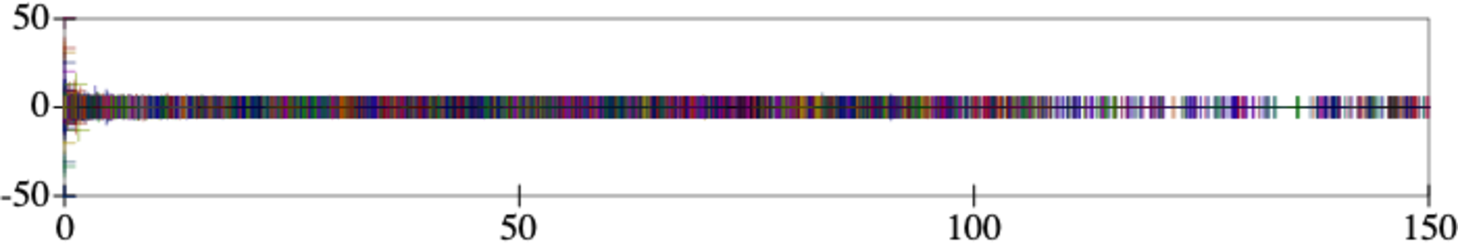
\includegraphics[width=\columnwidth]{img/error-count-nocheck-row--te-density-diff.pdf}
  \medskip
  \mnonstrict{}
  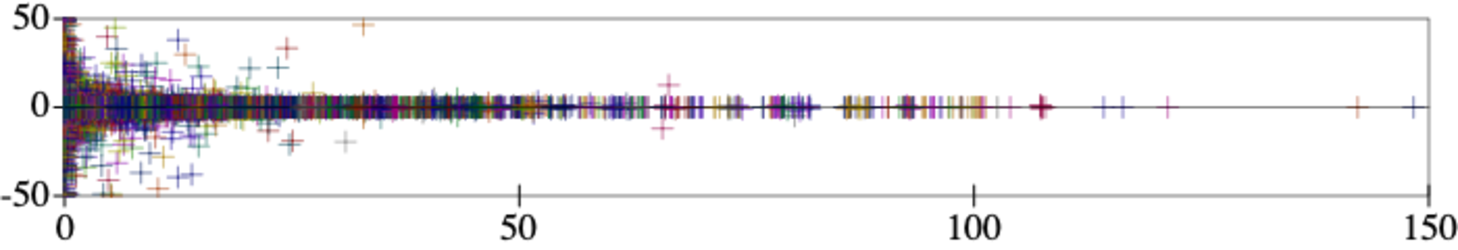
\includegraphics[width=\columnwidth]{img/error-count-nonstrict-row--te-density-diff.pdf}
  \medskip
  \mstrict{}
  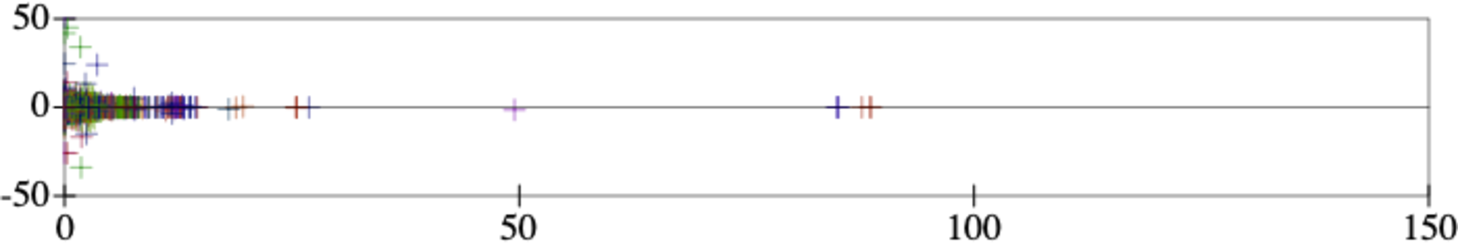
\includegraphics[width=\columnwidth]{img/error-count-strict-row--te-density-diff.pdf}
  \caption{Changes over time (seconds) to type error density (total errors / lines in project)}
  \label{f:error-density}
\end{figure}

\FILL{} what does the FS plot look like? is that a better nocheck-vs-rest comparison??

Moving on to type errors across the projects, and not just in the edit range,
a first interesting question is to study how the overall number of errors
changes over time.
But, the sheer number of errors can be skewed by codebase size.
To give a better basis for project-to-project comparisons, we focus
on the density of errors rather than the count, where \emph{density} is
the total number of type errors divided by the lines of code in the project.

\Cref{f:error-density} presents a zoomed-in view of type error density as it
changes over time in every session of the dataset.
The x-axis counts time in seconds from the start of the session.
The y-axis shows the change in density from the previous telemetry record
in the session to the next.
Changes can be positive or negative depending on whether the edits added
or removed errors.
The plots cut off at$\pm{}50$ density and 150 seconds.to focus on the
bulk of the data.
%% Sadly even with the zoom, it's too hard to follow one session ... the plot only gives a big-picture impression.


\paragraph{Observations}

Due to the relative adoption of type analysis, there is much more
data for the weak \mnocheck{} mode than for \mnonstrict{},
and in turn for \mnonstrict{} relative to \mstrict{}.
Still, the plots reveal interesting points:

\begin{itemize}
  \item
    All three plots are roughly balanced,
    with equal ``mass'' above and below the x-axis.
    The next section explores this point in detail.

  \item
    After the 40-second mark, changes to type error density become much
    smaller.
    Why?
    There are also fewer sessions (\mstrict{} makes that very clear).

  \item
    \mnonstrict{} has the biggest number of up/down deltas in the 10+ range.
\end{itemize}


\subsection{Do Edits Tend to Add Type Errors?}

\begin{figure}[t]\centering
  % TODO use bars instead, percent only, don't care about counts
  %% TODO old version had +-20% add/drop and a bigger % of keeps. What changed?
  \begin{tabular}{lr@{}rr@{}rr@{}r}
    & \zerowidth{Add} & & \zerowidth{Keep} & & \zerowidth{Drop} \\\midrule
    \mnocheck{} & 48378 & [\pct{46.83}] & 9440 & [\pct{9.14}] & 45479 & [\pct{44.03}] \\
    \mnonstrict{} & 19491 & [\pct{39.63}] & 9567 & [\pct{19.45}] & 20121 & [\pct{40.91}] \\
    \mstrict{} & 733 & [\pct{39.18}] & 368 & [\pct{19.67}] & 770 & [\pct{41.15}] \\
  \end{tabular}
  \caption{How often do edits increase, maintain, or decrease the number of type errors?}
  \label{f:error-changes}
\end{figure}

The apparent visual symmetry in the density plots~(\cref{f:error-density})
suggests that edits add and remove errors with rougly equal frequency,
regardless of mode.
No matter whether a creator is using \mnocheck{}, \mnonstrict{},
or \mstrict{} mode, edits seem to balance increases and decreases in the number
of type errors.
\Cref{f:error-changes} explores this question of balance in detail.
For each of the three modes, it reports the percent of edits that increase (Add),
maintain at a nonzero level (Keep), or decrease (Drop) the number of type
errors in the project.


\paragraph{Observations}

\begin{itemize}
  \item
    The Adds and Drops are remarkably balanced: across all three modes, they are
    at most \pct{2} apart from one another.
    This confirms that changes to the number of errors are balanced.
    Creators tend to fix errors highlighted by type analysis
    even in the stricter analysis modes.

  \item
    The percentage of Keeps is somewhat high: nearly \pct{10} in \mnocheck{}
    and \pct{20} in \mnonstrict{} and \mstrict{}.
    Evidently, the mode plays a role here.
    Outside of \mnocheck{}, type errors are more likely to persist through edits.

\end{itemize}


\subsection{Two Activities: Asset Creation and Scripting}

\begin{figure}[t]\centering
  %% TODO
  %% - thin bars
  %% - colors for good , bad (disagree) , neutral
  \begin{tabular}{lll}
    \mnocheck{} & \mnonstrict{} & \mstrict{} \\
    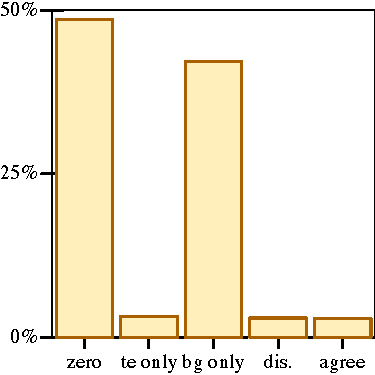
\includegraphics[width=0.3\columnwidth]{img/compass-nocheck.pdf}
    &
    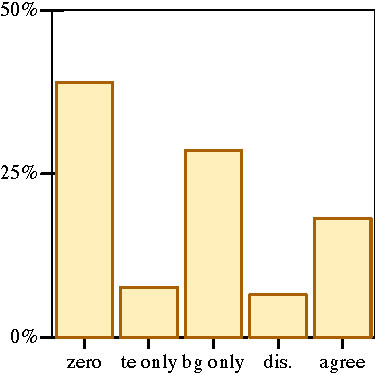
\includegraphics[width=0.3\columnwidth]{img/compass-nonstrict.pdf}
    &
    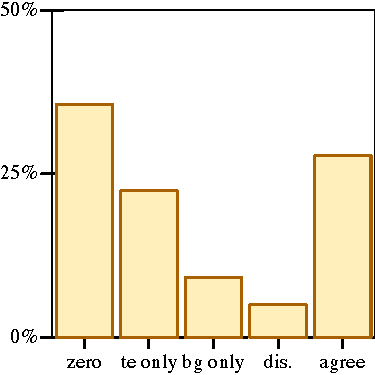
\includegraphics[width=0.3\columnwidth]{img/compass-strict.pdf}
  \end{tabular}
  \caption{FILL Are there fewer type errors than forcedstrict errors? Expect true always, but that is not the case.}
  \label{f:tefs-compass}
\end{figure}

Since Roblox Studio runs each codebase through two passes of type analysis,
it is interesting to compare their results.
Of special interest is the \mstrict{} mode case, because the number of
type errors and forced strict errors should be nearly the same.
But, there are two differences between \mstrict{} type checking
and forced strict checking:
\begin{itemize}
  \item
    Forced strict checks all dependencies in \mstrict{} mode, no matter
    what mode they declare.
    So, the number of forced strict errors may be higher.
  \item
    Forced strict has looser rules for the \emph{data model};
    that is, for the static assets that a program manipulates.
    So, the number of forced strict errors may be lower.
    %% initial DM, all properties go into a table type; DM -> folder -> model -> part
    %% get dot-driven autocomplete
\end{itemize}
Our data contains a surprising number of records where forced strict
reports fewer errors.
Data model edits are apparently a regular occurrence in Luau programs.

\Cref{f:tefs-compass} compares changes in type errors (\tekey{}) to changes in forced
strict errors (\fskey{}) for the three analysis modes.
To a first approximation, the changes either agree with one another
or disagree.
For example, if type errors increase but forced strict errors decrease,
we have a disagreement.
The plots futher categorize agreements and disagreements into
the following five cases:
\begin{enumerate}
  \item
    \emph{zero}: neither \tekey{} nor \fskey{} changed
  \item
    \emph{te only}: \tekey{} changed but \fskey{} remained the same
  \item 
    \emph{fs only}: \tekey{} remained the same but \fskey{} changed
  \item
    \emph{dis}: \tekey{} and \fskey{} changed in opposite directions
  \item 
    \emph{agree}: \tekey{} and \fskey{} changed in the same direction
\end{enumerate}
Both \emph{zero} and \emph{agree} are agreements.
The others are disagreements.
The plots show what percent of all telemetry records fell into these five categories.

\paragraph{Observations}

\begin{itemize}
  \item
    All three plots have a nonzero percentage of \emph{te only} items.
    In \mstrict{} mode, the percentage jumps up to nearly \pct{25}.
    Since \fskey{} is more lenient only for data model changes, these must
    be edits that affect the model in a way that raises a type error.
    Naturally, \mstrict{} mode has the largest number of such edits because
    its type checker is the most careful.

  \item
    In the first plot, for \mnocheck{},
    half the records are \emph{zero\/}s, nearly half are \emph{fs only}, and only a few
    land in the other categories.
    While the number of zeros is a bit high,
    the \emph{fs. only} spike makes sense because type checking is supposed to complain
    sparingly in \mnocheck{} mode.

  \item
    In the \mnonstrict{} plot, the number of agreements jumps up.
    This is reassuring.
    \FILL{}.

\end{itemize}

Users of \mstrict{} mode may find it frustrating that the type checker complains
about data model edits.
Though we cannot see the exact reason for the complaints, the checker errs on
the conservative side.
Thus we expect the number of useful reports is low.
This may be a barrier to adaption.


\subsection{Session Timelines}

\begin{figure}[t]\centering
  %% TODO any way to cluster timelines to avoid the "creepiness" of spying on one user?
%  \mnonstrict{}\\
%  \includegraphics[width=\columnwidth]{img/timeline-nonstrict.pdf}

  \medskip{}
  \mstrict{}\\
  \includegraphics[width=\columnwidth]{img/timeline-strict.pdf}

  \caption{Example sessions}
  \label{f:indy-session}
\end{figure}

Another insightful visualization that the telemetry supports is plots of individual sessions
over time.
\Cref{f:indy-session} shows the type errors, forced strict errors, and module switches
in two \mstrict{} mode sessions.
The x-axis shows time in seconds from the start of the session.
The y-axis counts errors.
Type errors appear as orange plus marks.
Forced strict errors appear as green x marks.
The vertical lines show module switches.

In the first plot, the error counts are low until about the 3,000s mark,
at which point an edit (not a module switch) leads to 15 errors.
These 15 errors disappear two records later.
Then, after two module switches and some edits, the number of errors spikes again.
In the second plot, the number of errors spikes in the beginning due to edits,
then remains low for the next few thousand seconds.

A general observation is that the number of type errors is always less than the number of forced strict
errors, though the numbers are close.
This should happen in \mstrict{} mode.


\section{Discussion}
\label{s:discussion}

\FILL{} good things first,
then regrets about the noisy stochiastic telemetry,
then lessons?
then threats.

\paragraph{Good: No Internal Error}

FILL hope to never see \code{InternalError}.
Have zero, yay!


\paragraph{Do Types Improve Quality of Life?}

\FILL{} compare \mnonstrict{} and \mstrict{}.
Use edit range~(\cref{t:type-error-survival} for NS vs S)
and error density~(\cref{f:error-delta})

TODO nocheck accumulated fs errors?



\paragraph{Bad: Noisy Data}

\begin{verbatim}
 require(foobar)
  foobar is a module script in the data model
 require(foo.bar.b)
  - could be edit in progress
  - could be renamed module
  - 
\end{verbatim}



\subsection{Threats to Validity}
\label{s:threats}

Error counts per-project and per-module include syntax errors.
Problematic, because syntax errors are uninteresting (easy to fix),
but common, which makes it likely that our per-keystroke telemetry (1/200) will record them.
Edit range has specific counts.
Next time, we should do that for the other aggregates.

Telemetry cannot replace user studies, as there is no way to measure
creator sentiment, but provide complementary data at scale.


\section{Related Work}
\label{s:related}

Liblit dissertation~\cite{liblit-thesis}

RAMSS workshop series.

Differential privacy for coverage analysis of software traces,
adds noise to traces,
hard because infinitely many traces,
use CFG abstraction of possible behaviors for callgraph analysis,
count sketch data structure~\cite{hlzbr-ecoop-2021}.

Nasko~\cite{zhlbr-cc-2020,zhlbr-oopsla-2020,hlzbr-ecoop-2021}

%% - zfstt-ieeesensors-2022
%% - lit review, benefits of static types
%%   http://danluu.com/empirical-pl/
%% - thomas kennedy .... generic usage monitoring ascilite 2003
%% - ahmadzadeh elliman higgins iticse 2005
%% - buffardi etal 2014 adaptive and social mechanisms
%% - bddf-icse-2016
%% -  sh edwards and jason snyder icer 2009 comparing effective and ineffective grading platform
%% - murphy etal sigcse 2009 Retina: helping students
%% - ESP workshop on empirical studies of programming
%%   https://dl.acm.org/doi/proceedings/10.1145/266399
%%   nothing sounds big ... empirical yes, large no
%% - Choppella Haynes IU TR 426
%% - Tip Dinesh tosem 2001

\cite{bgimgm-cse-2016}
study Java compiler error messages after an intervention, counting num errors,
counting repeats, counting per user

\cite{anna-russo-kennedy-ms-2006}
BitFit, web-based java ide log num hint requests num, result of check answer
requests num compile, num run, no code?! good we have the same constraint

\cite{ab-sigcse-2015}
frequency, time-to-fix, spread of errors
 (we can't do time)
parsing compile error + source code
 sometimes with custom parsers

\cite{m-masters-2016}
study errors in blackbox dataset,
 overwhelmingly syntax

\cite{bkmu-sigcse-2014}
blackbox, 100k users
source code, diffs
error line, column, message;
keep all comments EXCEPT one above the class declaration


\cite{bask-icer-2018}
2TB data, Java programs
18 publications survey, technical challenges in analysis
 most pubs analyze errors;
nobody asked:
 which exns do students encounter (what?! mccall kolling 2014)
 execution / editing timelines
(blackbox analysis tutorial in sigcse 2020 on a mini dataset, to help researchers start writing an analysis)


\cite{t-hatra-2021}
plan for a large user-centered study 
... not very deep, look at edit sequences, replay for errors


\cite{cdhhjklwya-hatra-2020}
evaluating the PLIERS design process (Coblenz etal 202X)
teaching students to use PLIERS; everyone ran a user study!
6 languages
 3 ran usability studies
recommend talk-alouds


\cite{gstf-hatra-2021}
liquid types for java
30 devs user study
 zoom

\cite{lfgc-pldi-2007}
typechecker never errors,
 calls a helper that looks for nearby programs that do typecheck
tested on
 10 students, 2yrs professional experience
 5 hw assignments
 2122 files collected;
won \pct{19}, lost \pct{17};
ill-suited for things like (let x = e1 in ....),
 change e1,
 use typechecker feedback to guide edits;
small data!


\cite{w-popl-1986}
reporting source, not detection
tested on 9 type errors
 all \emph{deletions}, such as forgetting to inject in an enum

\cite{sscwj-oopsla-2017}
NATE numerical analysis of type errors
5000 labeled programs
 errors from class, first fix


\cite{sjw-jfp-2018}
type error witness generation
4500 ill-typed student programs
 \pct{85} of time, synthesis works
 \pct{70} of time, locate source


\cite{h-dissertiation-2005}
constraint-based type inference;
general te criteria:
- target audience (novice / expert)
- output format (text / viz)
- interactivity (yes / no)
- heuristics (yes / no)
- primary-or-external (most type errors are easy, some could really use dedicated help)


\cite{hw-scp-2004}
location of type error as a slice,
 not a srcloc,
 not a subtree



\paragraph{Research on Errors}

TODO Liblit dissertiation

Mind your language~\cite{mfk-onward-2011}.


\paragraph{Telemetry}

\begin{table}[t]
  \caption{Comparing telemetry systems}
  \label{t:telemetry-design}

  \begin{tabular}{l@{~}cccccc}
    &             & PII       & Session ID & Deterministic & Private Data (???) \\\midrule
    & Transparent & \chkNo    & \chkNo     & \chkYes       & \chkNo      \\
  * & Us          & \chkNo    & \chkYes    & \chkNo        & \chkYes     \\
    & Diff.Priv   & $\epsilon$ & \chkYes   & \chkYes       & \chkYes     \\
    & Liblit      & ?         & ?          & ?             & ?           \\
    & \code{.NET} & \chkMaybe & \chkYes    & \chkYes       & \chkYes     \\
    & VS Code     & \chkYes   & \chkYes    & \chkYes       & \chkYes     \\
  \end{tabular}
\end{table}

Transparent telemetry: explain what it is and contrast our approach.
What essential, non-transparent things did we collect?

counting only, public decisions about what to count, public data,
collected weekly for a sample of clients, LastWeek field = prior day when
system gathered any data;
eg command invocations, lib stack frames, 
no user ID, no machine ID,
no time-ordered traces~\cite{transparent-telemetry}.

kindle track every tap (page turn etc),
enables whispersync feature,
drove design of navigation tools,
opt-out possible~\cite{kindle-telemetry}

vscode: usage data, crash reports, error data (not a crash but unexpected);
save file, open terminal, copy-paste, autocomplete offered, git queries, machine id,
session id, timestamp,
opt-out may be possible, but not for all usage data (per license, sec 2a) and
every extension can do its own thing~\cite{vscode-telemetry}

.NET SDK and .NET CLI:
crash reports, command invoked, args, hashed cwd, timings;
more listed online;
custom builds beware inadvertant disclosure, keep your filepaths clear;
data published in aggregate under CC-BY;
opt-out possible~\cite{dotnet-telemetry}


\cite{lnsmc-usenix-2018} blame-proportional logging,
scale up ``near'' points of interest,
could be useful for us in the future.
\cite{fnm-sigmod-2020} ditto, faster than statistical at finding root-cause,
deterministic.



\section{Conclusion}
\label{s:conclusion}

Quickly summarize findings:

\begin{itemize}
  \item
    \pct{50} of errors in current module, so probably errors appear locally (not in a distant module);
    \pct{5} of (current? old??) type errors overlap with edit range, so they don't stick around.
  \item
    \pct{90} \mnocheck{},  \pct{10} \mnonstrict{},  \pct{0.1} \mstrict{}, wow.
  \item
  \item
  \item
    DM awareness is an important and surprising gap between strict
    and forced strict, undoubtedly a usability barrier for \mstrict{}.
  \item
\end{itemize}

Quick regrets, lessons learned, advice for next time

\paragraph{Future work: Low adaption}

why so few using nonstrict and strict?
needs advertising?
needs usability?


\paragraph{Do we need timestamps?}

FILL these were helpful for the overview

Our telemetry records include timestamps.
While timestamps are not personal data per se, they are in the ballpark.
Telemetry would be even more private without them.
Do we need them?

Timestamps are not the focus of our analysis, but they do play a critical role.
Consider~\cref{f:error-delta}.
With timestamps, it is clear that error density stays close to zero.
Without timestamps, we would be left with the counts at the bottom
of~\cref{f:error-delta}.
Many distributions could fit those counts, such as a ``mountain'' session that first
grows and grows the number of type errors then shrinks and shrinks down to zero.


\acks

Thanks to Benjamin Chung for several helpful discussions about data analysis
and effective plotting.
Greenman was supported by
grant \href{https://nsf.gov/awardsearch/showAward?AWD_ID=2030859&HistoricalAwards=false}{2030859}
to the CRA for the \href{https://cifellows2020.org}{CIFellows} project.

\newpage

\appendix

\section{Data Details}

Tips for interpreting the data:

\begin{itemize}
  \item
    Edit ranges are non-negative because we
    implemented the interval arithmetic for them using unsigned integers.
    To filter out negative edit ranges, we removed all ranges
    greater than 4 billion.

  \item
  \item
  \item
\end{itemize}

\newpage

\bibliography{bib}

\end{document}
